\subsection{Configuration File}

All devices in the research allow a configuration file to be exported and later imported. These configuration files expose additional settings that are not available through the management interfaces. Most of the \glspl{cpe} export it as plaintext, but \glspl{cpe} 3, 5, and 7 encrypt the file. Some fields of the file exported from \gls{cpe} 2 are also encrypted.

The fields encrypted on \gls{cpe} 2 configuration file are hex-strings prefixed by \texttt{\_encrypted\_}. When decoding the strings, it always started with the characters \texttt{A}, \texttt{E}, \texttt{S}, and \texttt{\textbackslash0}, indicating that \gls{aes} is the cipher used to protect the original content. It was detected that the same value was encrypted twice in the configuration file producing distinct ciphertexts, indicating that either different keys are used to encrypt different fields or the key is salted upon encryption. Unfortunately the decryption key was not found and it is unknown. 

The encryption used on \glspl{cpe} 3 and 7 was identified by binwalk \cite{binwalk} to be OpenSSL with a salted password. Just like on \gls{cpe} 2, the key could not be identified.

\gls{cpe} 5 was different, the exported configuration file carries plaintext data mixed with ciphertext data. Originally it was speculated that the file was using some non-standard compression algorithm as binwalk wasn’t able to identify the file type. But there is a tool that can be used to decode the configuration file when accessing the device via \gls{ssh} or Telnet, and after decoding the exported file, it became smaller. So the file was indeed encrypted and not compressed. While the tool allowed the file to be modified and restored on the device, the decryption binary cannot be executed outside the device, as it communicates with a character device managed by an unknown kernel module. But by decompiling the binary and their dependencies using Binary Ninja \cite{binary_ninja} and Ghidra \cite{ghidra}, it was able to recover the encryption and decryption algorithm used by the \gls{cpe}, as shown in Figure \ref{figure:libaspcm_so}. By simply adding or removing a 16-byte header from the configuration file and XORing every byte with 8, the file can be encrypted or decrypted. The decryption function, reimplemented in Python, is available on Appendix \ref{appendix:cpe_config_file_dec}.

\begin{figure}[h]
    \centering
    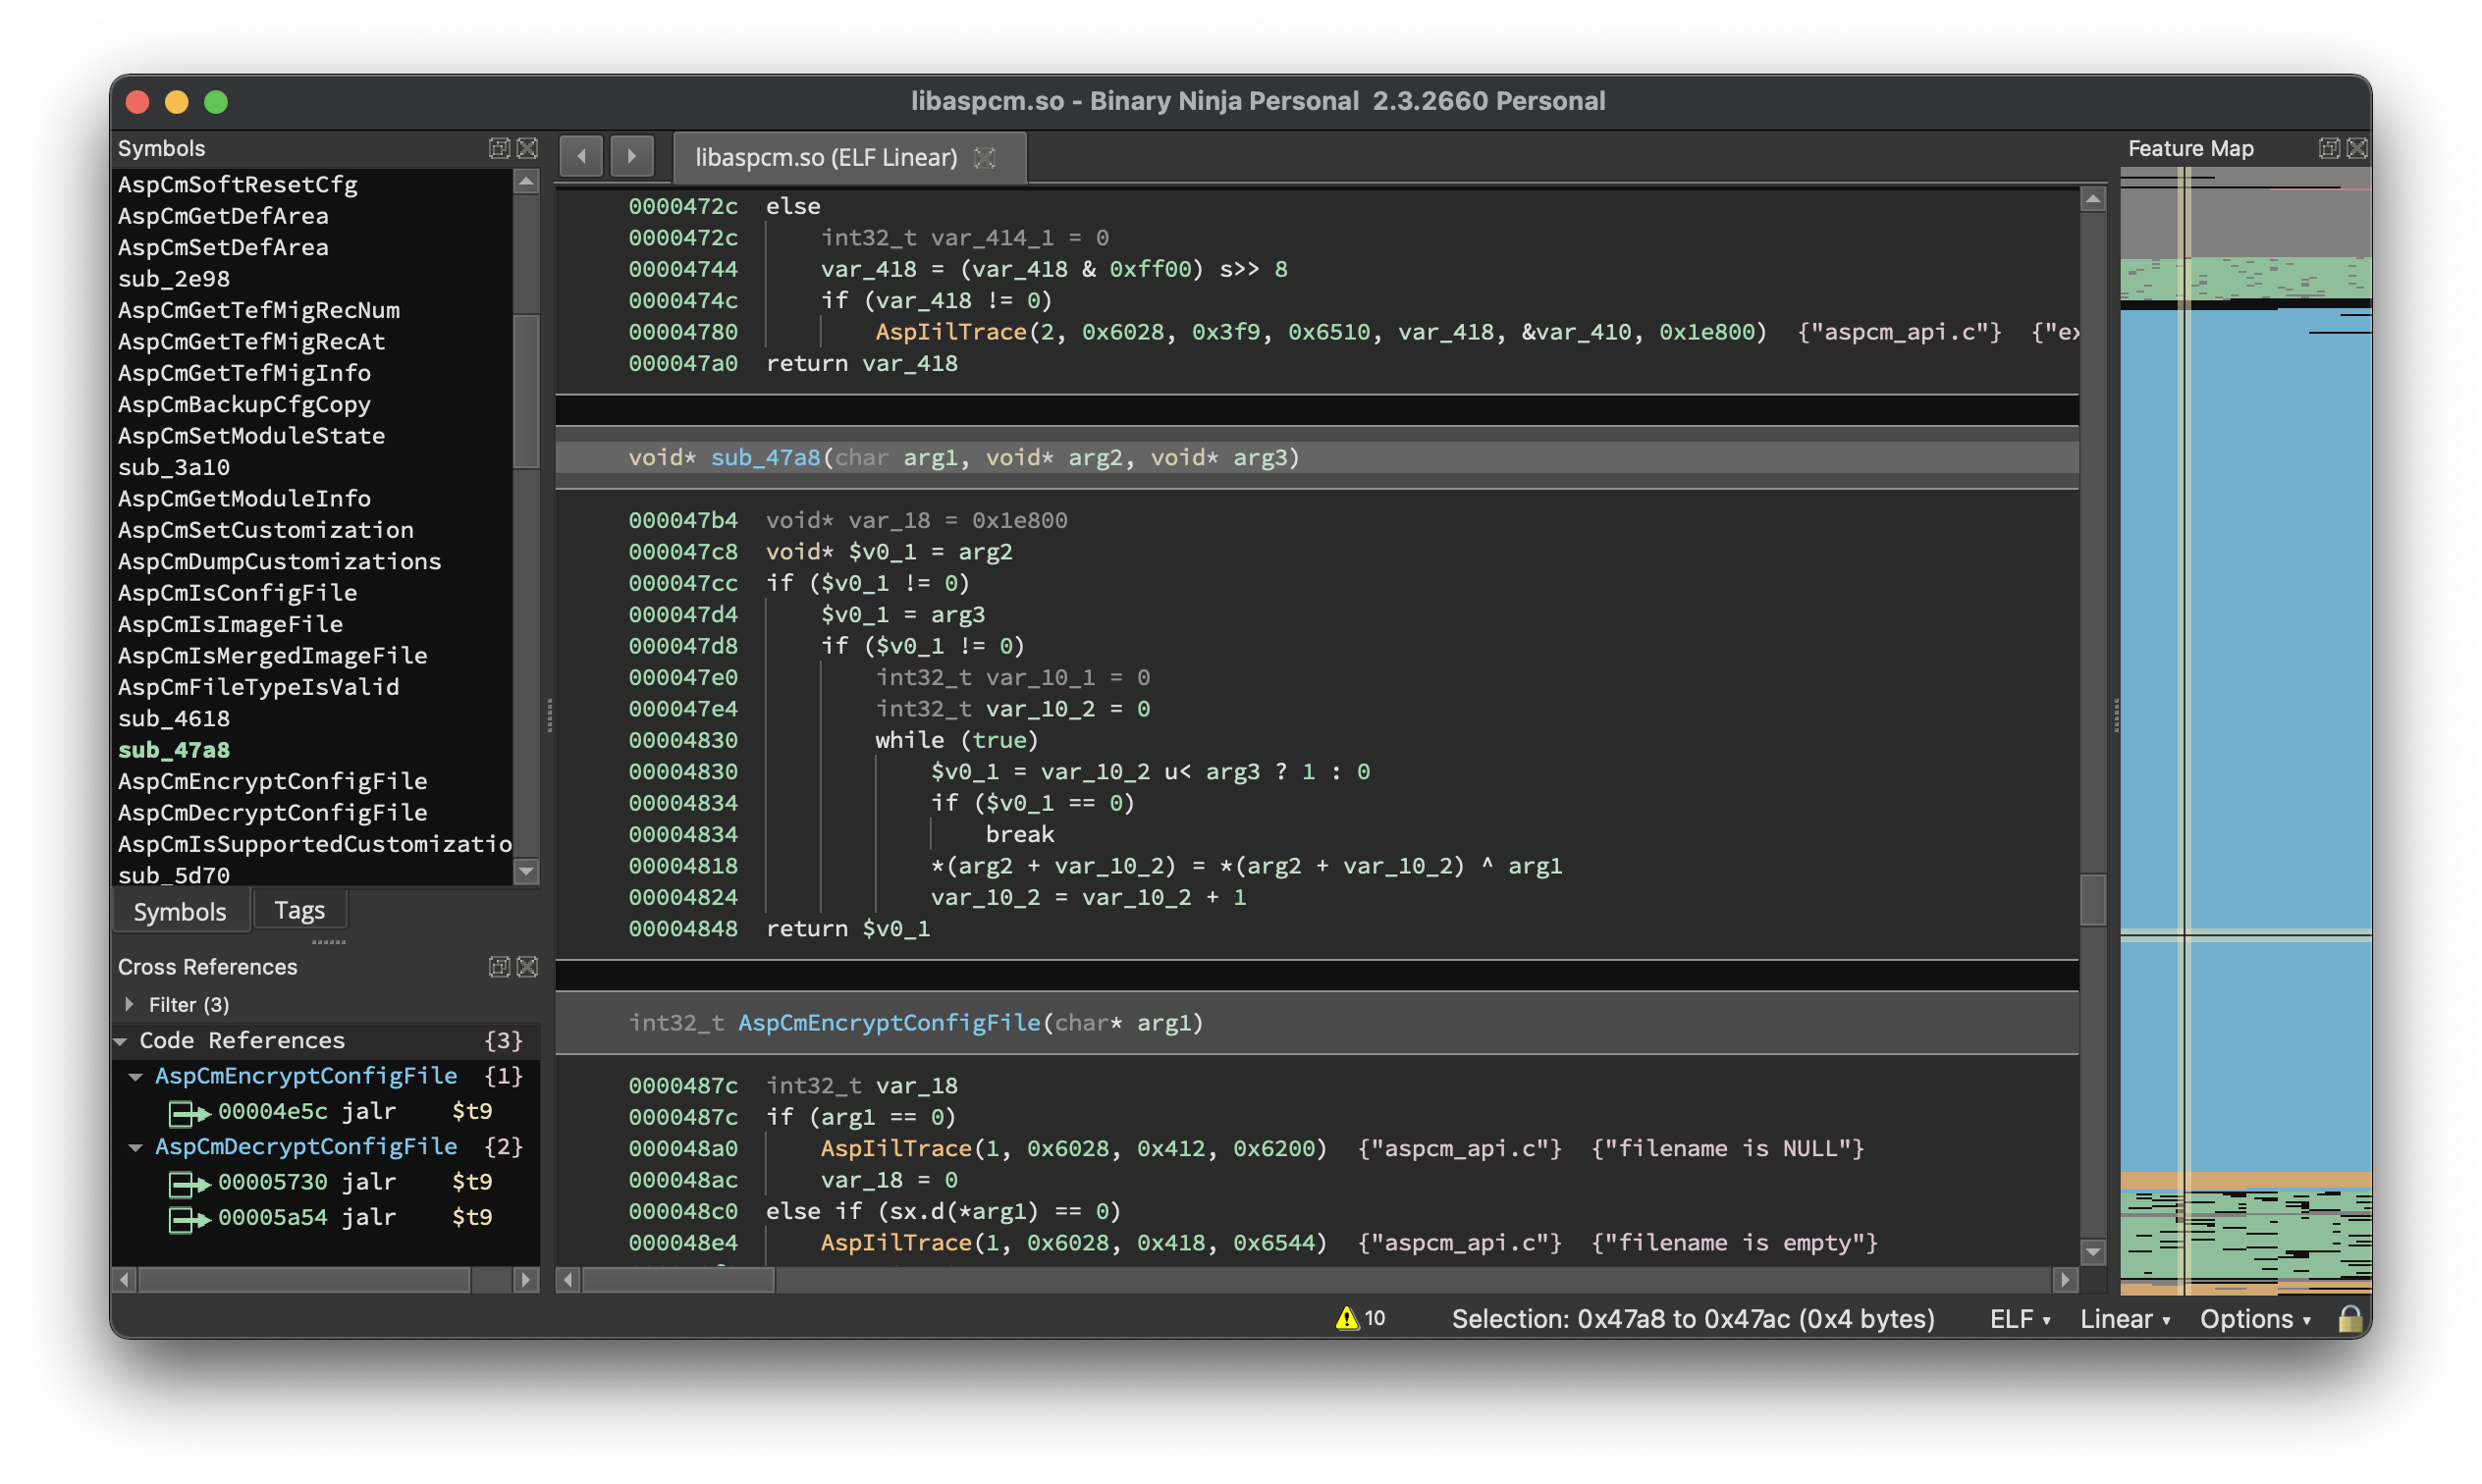
\includegraphics[width=\linewidth]{contents/configuration-analysis/configuration-file/libaspcm-so.png}
    \caption{Function \texttt{sub\_47a8} of \texttt{libaspcm.so} Decompiled by Binary Ninja}
    \label{figure:libaspcm_so}
\end{figure}

\FloatBarrier
